%%%%%%%%%%%%%%%%%%%%%%%%%%%%%%%%%%%%%%%%%%%%%%%%%%%%%%%%%%%%%%%%%%% 
%                       rpithes-short.tex                         %
%         Template for a short thesis all in one file             %
%        (titlepage info below assumes masters degree}            %
%  Just run latex (or pdflatex) on this file to see how it looks  %
%      Be sure to run twice to get correct TOC and citations      %
%%%%%%%%%%%%%%%%%%%%%%%%%%%%%%%%%%%%%%%%%%%%%%%%%%%%%%%%%%%%%%%%%%% 
%
%  To produce the abstract title page followed by the abstract,
%  see the template file, "abstitle-mas.tex"
%
%%%%%%%%%%%%%%%%%%%%%%%%%%%%%%%%%%%%%%%%%%%%%%%%%%%%%%%%%%%%%%%%%%%

\documentclass{thesis}
\usepackage{graphicx}   % if you want to include graphics files
\usepackage[draft]{todonotes}

\newcommand{\comment}[1]
{\par {\bfseries \color{blue} #1 \par}} %comment showed

% Use the first command below if you want captions over 1 line indented.
% A side effect of this is to remove the use of bold for captions. 
% To restore bold, also include the second line below.
%\usepackage[hang]{caption}     % to indent subsequent lines of captions
%\renewcommand{\captionfont}{\bfseries} % only needed with caption package;
                                        %   otherwise bold is default)


%%%%%%%%%%%%%%%%%%%%  supply titlepage info  %%%%%%%%%%%%%%%%%%%%%
\thesistitle{\bf Performance of heterogenous networks of AMQP1.0 compliant Message-orientated Middleware (MOM) brokers}        
\author{David Joe Wade}        
\degree{Master of Science}
\department{Computer Science} 
\thadviser{Dr. Eugene Eberbach}
%\cothadviser{First co-adviser} %if needed
%\cocothadviser{Second co-adviser} % if needed
%  For a masters project use \projadviser instead of \thadviser, 
%  and \coprojadviser and \cocoprojadviser if needed. 
\submitdate{April 2014\\(For Graduation May 2014)}        

%%%%%%%%%%%%%%%%%%%%%   end titlepage info  %%%%%%%%%%%%%%%%%%%%%%
      
\begin{document} 
\listoftodos
\titlepage            	 % Print titlepage          
\tableofcontents          % required 
\listoftables          	 % required if there are tables
\listoffigures         	 % required if there are figures

\specialhead{ACKNOWLEDGMENT}
Special thanks to my wife Anne, my son Jack, and my daughter Erin - sorry for the added stress while putting this together.  I also have a great amount of gratitude to my parents, Brian and Catherine - who helped keep the family running while I focused on this project.

\specialhead{ABSTRACT}
The Advanced Message Queuing Protocol (AMQP) provides an open standard protocol for message orientated middleware (MOM).  There are currently many different AMQP compliant MOM implementations, both open-source and proprietary.  

Because of this standard it is possible to integrate different implementations have been developed that meet the AMQP standard - making it possible to integrate disassociated systems without having to standardize MOM implementations across different teams.  \todo{reword}  

This paper provides benchmarking information about performance impact of integrating different AMQP implementations.  

\chapter{INTRODUCTION}

\section{Middleware}
In computer science, the term \"middleware\" has many meanings.  Generically, middleware can be thought as \"glue\"  for computer software.  It facilitates communication between different software components - abstracting the complexities of intra and inter process communication from a software developer to allow focus on the core functionality of a software component.  In a broad sense, things such as user space software drivers, virtual machines and kernel IPC are forms of middleware.  This paper focuses on middleware as it relates to distributed applications - typically used to share data and state between software components that exists in separate execution environments connected though a network.

Even with this narrow definition there are many different architectures for data passing/communication.  Some of the common design patterns used are: enterprise application integration (EAI), data integration (DI), message oriented middleware (MOM), object request brokers (ORB) and the enterprise service bus (ESB).  

\subsection{Message Oriented Middleware (MOM)}
Message-orientated middleware (MOM) is software that facilitates the development of distributed systems by providing an infrastructure for asynchronously sending and receiving data over a network \cite{todo}.   There are many implementations of such messaging systems, but until recently most of them have been closed source/proprietary systems.  Lacking any standard for communications protocols software, developers and systems engineers were often forced to choose (or have chosen) a single MOM implementation and become stuck with its features and limitations.  

\todo{describe other middleware systems, CORBA, DDE, etc}
\todo{what are the fundamental types of middleware (data-centric, object-orientated, message-oriented)}

\section{AMQP History}
The development of AMQP was started in 2003 by John O'Hara and others at JPMorgan Chase in London, UK.  JPMorgan was looking for a messaging solution with high durability that supported a very high number of small message transactions (in the range of 500,000 messages/second) \cite{todo}.  Initial development was done internally at JPMorgan Chase but was later subcontracted with iMatix Corporation for a broker and protocol documentation.  In 2005 JPMorgan Chase formed a working group with other companies such as: Cisco Systems, Red Hat, iMatix and the Transaction Workflow Innovation Standards Team (TWIST).

The working group released four major versions of the AMQP standard:
0-8 published in June 2006
0-9 published in December 2006
0-9-1 published November 2008
0-10 published in February 2008
1-0 published October 2012

\subsection{AMQP 1.0}

Version 1.0 was a major departure from the previous AMQP versions and caused significant backlash among the AMQP community.  Even two years after the formal adoption of the AMQP 1.0 specification there are major broker implementations (e.g. RabbitMQ) that do not directly support the AMQP 1.0 standard.  

\subsection {Specific differences}

AMQP 0-10 specified the wire-level protocol and a broker architecture.  AMQP 1.0 only specified a protocol specification and does not impose the traditional AMQP architecture (bindings, exchanges, queues, etc) of earlier specifications.  

AMQP 1.0 is symmetric - it places no constraints on roles of connections endpoints.  Previous AMQP versions had strict definitions for clients and brokers.  Every connection must have a defined client and server (broker).  The AMQP 1.0 standard is much more flexible, it permits point-to-point connections where no central broker or broker network is part of the data transfer.  

AMQP versions before 1.0 also specified protocol commands to manage brokers.  AMQP 0-10 specifies commands such as "Create Queue", "Delete Queue", etc.  AMQP 1.0 does not define these messages as part of the protocol.


 

\todo{clean up format and cite}

JPMorgan Chase collaborated with Red Hat to develop the Apache Qpid MOM implementation.  Independently, RabbitMQ was developed by Rabbit Technologies as well as AMQP complient implementations by Microsoft and StormMQ.

The working group expanded to include 23 companies, including: Bank of America, Barclays, Credit Suisse, Deutsche B$\ddot{o}$rse Systems, Goldman Sachs, Microsoft Corporation, Novell, Red Hat, VMware and others.

The AMQP standard also defines message orientation, queuing, routing, reliability, and security.   AMQP also describes the wire-level format of the data so that any nodes that are AMQP compliant can handle the message stream.  

Standardization lead to the rapid development of many MOM systems such as: Apache Qpid, RabbitMQ, StormMQ, ActiveMQ, Apache Apollo, SwiftMQ.  Even Microsoft supports the AMQP1.0 protocol with their implementation of the ServiceBus class in .NET  and is a supported protocol on the Azure cloud computing platform.  

MOM implementations that support the AMQP version 1.0 specification (Released October 29th 2012) \cite{todo} are interoperable and are available on many platforms.  

\todo{describe AMQP version issues}

Because these implementations were designed around the message traffic of the financial services sector they excel at passing small messages and focus on message throughput.  There are performance differences between each implementation and generic benchmarks for each implementation are available \cite{todo}\cite{todo}.


\section{Alternatives}
The AMQP specification is not unique in its goal of providing a cross-platform, ubiquitous message protocol.  There are several popular specifications in current use.  Many MOM implementations that support the AMQP protocol also support these other protocols; some are built in natively while others need to be enabled as plugins.   

\subsection{STOMP}
Simple Text Oriented Message Protocol (STOMP) is a text-based protocol designed to work with message oriented middleware systems.  It defines a wire-level message encoding format that allows for STOMP clients to communicate with any STOMP enabled message broker.  It is built on top of TCP/IP and uses a protocol similar to HTTP.  

\subsection{OpenWire}
\todo{fill in section}

\subsection{XMPP}
Extensible Messaging and Presence Protocol
\todo{fill in section}

\subsection{MQTT}
MQ Telemetry Transport (MQTT) is a light-weight messaging protocol.  It is specifically targeted for applications where a light-weight protocol is needed due to code size limitations.  The protocol was invented by Andy Stanford-Clark (IBM) and Arlen Nipper (Cirrus Link Solutions).  

In 2013 the MQTT protocol specification was submitted to the OASIS specification body.  There is a variation of the standard (MQTT-S) for embedded applications on non-TCP/IP networks such as ZigBee.  Facebook Messenger uses the MQTT protocol internally for large parts of its functionality. 

%\todo{http://en.wikipedia.org/wiki/MQ_Telemetry_Transport}

\subsection{Java Messaging Service (JMS)}
The Java EE JMS (Java Messaging Service) was the starting point for attempting to standardize MOM. Unfortunately, JMS only specifies an application programming interface (API) and does not specify a format for exchanged messages so it does not create interoperability.   To achieve this desired interoperability other standards such as AMQP (Advanced Message Queuing Protocol) built upon the JMS standards). 



\section{AMQP Specification}


\section{AMQP implementations}

%\todo{comparision table with all chosen AMQP implementations (client languages/implementation/version/etc)}

\subsection{RabbitMQ}
RabbitMQ is an open source message broker written in the Erlang programming language.  \todo{http://www.rabbitmq.com} RabbitMQ is developed by and supported by Rabbit Technologies Ltd.  It is actively being developed, the latest stable version (3.2.4) was released on March 4, 2014.  It is licensed under the Mozilla Public License \cite{rabbitmq-wikipedia}.

The development history/management of RabbitMQ is complicated.  Originally developed by Lshift, the project was moved to an independent company Rabbit Technologies Ltd, which was cofounded by Monadic and CohesiveFT.  In 2013, Rabbit Technologies Ltd. was acquired by SpringSource, a division of VMware, Inc. \todo{http://www.lshift.net/blog/2010/04/13/rabbitmq-2}.  As of March 2014 - commercial support for RabbitMQ was being provided by Pivotal, Ltd \todo{http://www.gopivotal.com/support} \todo{work out relationship with VMware}.

RabbitMQ is cross platform and has bindings/clients for a wide range of systems/programming languages.  \todo{http://www.rabbitmq.com/devtools.html}.  has bindings/client for many different languages.  RabbitMQ has comprehensive documentation, and supports Clustering, High Availability, SSL, Management, etc. \todo{complete}


\subsection{ActiveMQ}
ActiveMQ is an open source message broker written in Java.  ActiveMQ is developed by the Apache Software Foundation and as of \todo{date} the most recent stable version is 5.9.0 released on October 21, 2013.

ActiveMQ is part of Apache's enterprise service bus (ESB) implementations, and is leveraged in other project such as Apache Camel and Apache CXF to Service Orientated Architecture (SOA) projects.

Version 5.3 of Apache ActiveMQ has published performance results using the SPECjms2007 benchmark. \todo{citation needed} 

%\todo{ http://en.wikipedia.org/wiki/ActiveMQ}

\subsection{ApolloMQ}
ApolloMQ is an open source message broker written in Java.  It is a fork of Apache ActiveMQ with the primary difference being the threading model and message dispatching architecture \todo{https://activemq.apache.org/apollo/}.  ApolloMQ maintains multi-protocol support and supports STOMP, AMQP 1.0, MQTT, OpenWire, SSL and WebSockets.



\subsection{HornetQ}
HornetQ is an open source, multi-protocol messaging system developed from JBoss, a division of Red Hat, Inc. \cite{http://en.wikipedia.org/wiki/JBoss_(company)}.  It can be integrated with JBoss Application Server or embedded into standalone applications.  As of version \todo{find version} it supports the AMQP1.0 specification.  HornetQ is released under the Apache Software License version 2.0 \todo{citation needed}.  There are a few components that are released under LGPL \todo{citation needed} but the plan is to develop a pure ASL2.0 version in the future.  HornetQ is written in Java and supports and platform with a Java 5 or later runtime.   It is actively being developed and maintained with the last stable version 2.4.0 being released on December 16, 2013 

%\todo{http://www.jboss.org/hornetq}

Tim Fox started the HornetQ project in 2009 and led the project until the end of 2010. 

HornetQ supports many important features.  It supports the STOMP \todo{how does this compare to AMQP} protocol and is 100\% JMS compliant.  It supports clustering for scalability and reliability and master/slave architecture for fault tolerance.  It leverages the high-performance Netty NIO connector over TCP and SSL.  The documentation for HornetQ is comprehensive and up to date.  

As of \todo{date} HornetQ holds the SPECjms2007 benchmark record \todo{citation needed}.  

%\todo{http://en.wikipedia.org/wiki/HornetQ}


\subsection{NullMQ}

\chapter{Methodology}
Marsh, Sampat, Potluri, Panda in [3] developed broker network architectures and benchmarked to support large federated broker networks and benchmarked the messaging passing performance.  They experimented with multi-level broker architectures and multi-consumer fanout patterns to find the optimal broker design patterns.  All of their work was performed with Apache Qpid implementation [3].  

Subramoni, Marsh, Narravula, Lai and Panda in [1] designed and developed benchmarks for MOM broker networks building using the Message Passing Interface (MPI) benchmarks developed by Ohio State University Network-Based Computing Laboratory’s [1] and the Standard Performance Evaluation Corporation (SPEC) MOM benchmarks  [1].  Benchmarks such as the Direct Exchange - Single Publisher Single Consumer (DE-SPSC) and Direct Exchange - Multiple Publishers Multiple Consumers (DE-MPMC) benchmarks [1] will be implemented for each AMQP implementation 

This project will combine the methodologies used in these experiments and add an additional variable, different broker implementations to determine what the performance impact of a heterogenous broker network on messaging performance.

In addition to these benchmarks, additional information will be collected in order to compare the performance of the broker implementations.

A lab environment will be setup to isolate the tests from outside message traffic.  High-end workstation, class laptop computers and business class network equipment will be used.  The computers will use the latest Long-Term Support version of the Ubuntu Server operating system (12.04LTS) and will be configured to minimize background daemons and processes.  The times of all systems will be synchronized using a local NTP server. A complete listing of software versions used will be published with the results of this research.

\subsection{Existing Benchmarks}
There are other existing and published benchmarks for MOM systems.  The most widely known is SPECjms2007 \todo{http://www.spec.org/osg/jms2007/}.  It was the first industry standard benchmark for evaluating the Java Messaging Service (JMS).

SPECjms2007 is designed to model a messaging system of a grocery store - it simulates all of the messages needed to maintain inventory/purchasing/etc.  It does this to provide a comprehensive - real-world evaluation of a messaging system.  The benchmark was expanded by \todo{find name and reference} to originally benchmark the Apache Qpid MOM system \{citation needed}.  The benchmark needs to be licensed from the SPEC organization.  

\subsection{Developed benchmarks}

The design of the benchmarks for this experiment we modeled after the work done by Subramoni, Marsh, Narravula, Lai and Panda in \cite{Subramoni} which in turn based their benchmarks on Ohio State University Micro-benchmarks \todo{citation needed}.  

\subsection{Direct Exchange - Single Publisher Single Consumer (DE-SPSC)}
\subsection{Direct Exchange - Multiple Publishers Multiple Consumers (DE-MPMC)}
\subsection{Single Publisher - Multiple Consumer (SPMC)}
\subsection{Topic Exchange - Single Publisher Single Consumer (SPSC)}

\missingfigure{something}

\chapter{Experimental Results}
\subsection{Experimental Setup}
And so on, for more chapters.
Another citation for the bibliography:\cite{anotherbook}

   This is a sentence to take up space and look like text.
   This is a sentence to take up space and look like text.
   Please refer to Figure~\ref{Figure 1}.  % Note \label command below

 
\begin{figure}
\centering
\vspace{2.0in} 
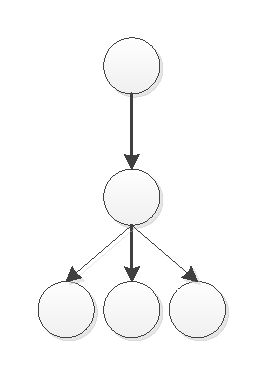
\includegraphics{Drawing4}  
\caption{This is the Caption for Figure 1 make it long to illustrate
   how it looks when wrapped around to the next line}
\label{Figure 1}  % the \label command comes AFTER the caption
\end{figure}


\begin{table}
\caption{This is the Caption for Table 2}
\label{mytable}
\begin{center}
\begin{tabular}{lll}
Here's	& another 	& example \\
of		& something	& useful \\
\verb+table+ & environment & command. \end{tabular}
\end{center}
\end{table}

% The following produces a numbered bibliography where the numbers
% correspond to the \cite commands in the text.
\specialhead{LITERATURE CITED}
\begin{singlespace}
\begin{thebibliography}{99}

\bibitem{thisbook} This is the first item in the Bibliography.
Let's make it very long so it takes more than one line.
Let's make it very long so it takes more than one line.
\bibitem{anotherbook} The second item in the Bibliography.

\bibitem{ActiveMQ} B. Snyder, D. Bosanac, R. Davies, "ActiveMQ in Action", Manning, 2011 pp 1 – 326.

\bibitem{Scaling AMQP} G. Marsh, A. Sampat, S. Potluri, D. Panda, "Scaling Advanced Message Queueing Protocol (AMQP) Architecture with Broker Federation and InfiniBand", Department of Computer Science and Engineering, The Ohio State University

\bibitem{Chirino} H Chirino, "STOMP Messaging Benchmarks: ActiveMQ vs Apollo vs HornetQ vs RabbitMQ", http://hiramchirino.com/blog/2011/12/stomp-messaging-benchmarks-activemq-vs-apollo-vs-hornetq-vs-rabbitmq/

\bibitem{Sachs} K. Sachs, K. Samuel, and S. Appel, "Benchmarking of Message-Oriented Middleware", ACM, pp. 1–2, Sep. 2009.

\bibitem{Subramoni} H. Subramoni, G. Marsh, S. Narravula, P. Lai, D. Panda, "Design and Evaluation for Financial Applications using Advanced Message Queuing Protcol (AMQP) over InfiniBand", Department of Computer Science and Engineering, The Ohio State University.

\bibitem{Maheshwari} P. Maheshwari and M. Pang, “Benchmarking Message-Oriented Middleware – TIB/RV vs. SonicMQ,” Journal Concurrency and Computation: Practice and Experience - Foundations of Middleware Technologies, vol. 17, no. 12, pp. 1507–1526, Oct. 2005.

\todo{Not sure if I really want to advertise this. How on Earth am I going to actually support this}
NOTE: Printed copies of all sources are available upon request. 

\end{thebibliography}
\end{singlespace}




\todo{Other sources - not sure if they are used anymore}
%
%J. Kramer, “Advanced Message Queuing Protocol (AMQP)”, Linux Journal, 11/1/2009, http://www.linuxjournal.com/%magazine/advanced-message-queuing-protocol-amqp
%
%G. Mazza, “FUSE Message Broker Performance Tuning Guide”, 8/31/2007, http://fusesource.com/wiki/display/
%ProdInfo/FUSE+Message+Broker+Performance+Tuning+Guide
%
%ActiveMQ Performance Module, http://activemq.apache.org/activemq-performance-module-users-manual.html
%
%
% P. Farrell and H. Ong, “Communication Performance over a Gigabit Ethernet Network.,” Performance, Computing, %and Communications Conference, pp. 1–9, Feb. 2004.
%
%
%Freeman, E. (1996). Middleware: Link everything to anything. Datamation, 42(16), 119-119. Retrieved from http://%search.proquest.com/docview/220221663?accountid=37764
%
%Q. Mahmoud, “Getting Started with Java Message Service (JMS), 11/2004, http://java.sun.com/developer/%technicalArticles/Ecommerce/jms/index.html
%


%%%%%%%%%%%%%%%%%%%%%%%  For Appendices  %%%%%%%%%%%%%%%%%%%
\appendix    % This command is used only once!
\addtocontents{toc}{\parindent0pt\vskip12pt APPENDICES} %toc entry, no page #
\chapter{THIS IS AN APPENDIX}
Note the numbering of the chapter heading is changed.
This is a sentence to take up space and look like text.
\section{A Section Heading}
This is how equations are numbered in an appendix:
\begin{equation}
x^2 + y^2 = z^2
\end{equation} 

\chapter{THIS IS ANOTHER APPENDIX}
This is a sentence to take up space and look like text.

\end{document}
